%%%% Opcje
%% wmii --- Wydział Matematyki i informatyki
%%
%% Kierunek:
%%      inf --- Informatyka
%%
%% Poziom studiów (praca):
%%      mgr --- magisterska

\documentclass[wmii,inf,mgr]{uwmthesis}

\newcommand{\version}{0.0.1}

\usepackage[MeX]{polski}
\usepackage[utf8]{inputenc}
\usepackage{url}
\usepackage{graphicx}
\graphicspath{ {./img/} }
\date{2017}
\title{Webowy system rozpoznawania odręcznie pisanych cyfr.}
\author{Wojciech Baczewski}
\etitle{Web system of recognizing handwritten digits.}
\wykonanaw{katedrze Metod Matematycznych Informatyki}
\ewykonanaw{Chair of Mathematical Methods of Informatics}

\podkierunkiem{dr Krzysztofa Sopyły}
\epodkierunkiem{dr Krzysztof Sopyła}

\begin{document}

\maketitle

\tableofcontents

\chapter*{Wstęp}

Wstęp


\chapter{Wykorzystane technologie}
\section{Java}


\section{Spring}
\section{Spring Boot}
\section{Maven}
\section{HTML}
Opis canvas

\section{IntelliJ IDEA}
\section{PostgreSQL}
\section{Apache Tomcat}

\chapter{Specyfikacja wymagań}
\section{Przypadki użycia}
\subsection{Diagram przypadków użycia}

\begin{figure}[!ht]
  \centering
    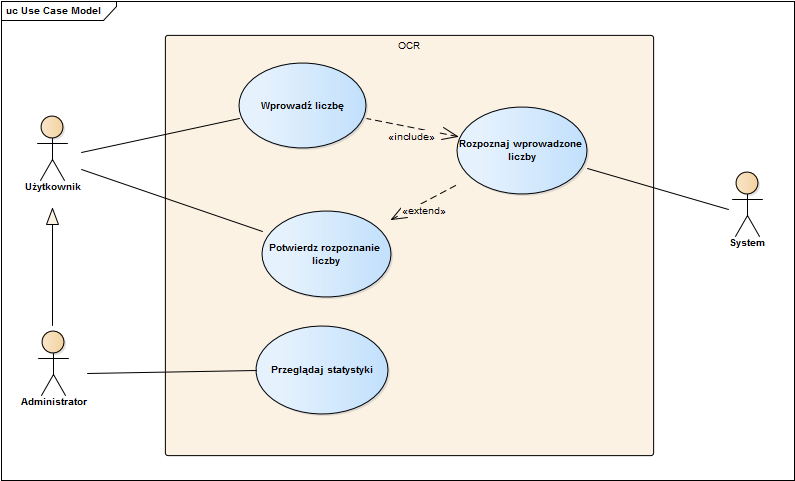
\includegraphics[scale=0.6]{UseCaseModel.png}
	\caption{Diagram przypadków użycia}
\end{figure}

\subsection{Scenariusze przypadków użycia}
\section{Diagram sekwencji}
Opis
\begin{figure}[ht]
	\centering
		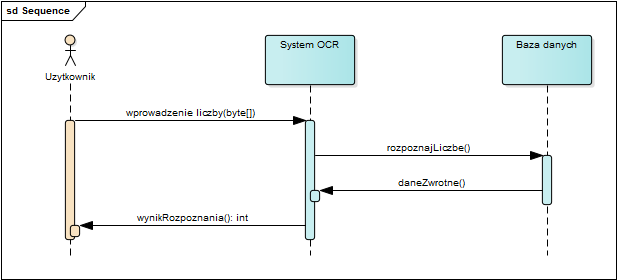
\includegraphics[scale=0.6]{Sequence.png}
	\caption{Diagram sekwencji rozpoznania wprowadzanych danych}
	\label{fig:Sequence}
\end{figure}

\section{Diagram klas}
\section{Diagram DDL}

\chapter{Metoda klasyfikacji}

TODO: research. (SVM,Convolution(CNN)) 
Opis wybranej metody klasyfikacji

\section{Opis algorytmu}

\chapter{Implementacja}
\chapter{Opis interfejsu użytkownika}
Zrzuty ekranu z aplikacji albo mockup
\chapter*{Instrukcja instalacji oprogramowania}

\chapter*{Spis rysunków}
\chapter*{Spis diagramów}
\chapter*{Spis Tabel}
\thebibliography{1}

\chapter*{Podziękowanie}

\begin{streszczenie}

\end{streszczenie}

\begin{abstract}

\end{abstract}

\end{document}
